\documentclass{ieeeaccess}
\usepackage{amsmath,amssymb,amsfonts}
\usepackage{graphicx}
\usepackage{textcomp}

\usepackage{bm}
\makeatletter
\AtBeginDocument{\DeclareMathVersion{bold}
\SetSymbolFont{operators}{bold}{T1}{times}{b}{n}
\SetSymbolFont{NewLetters}{bold}{T1}{times}{b}{it}
\SetMathAlphabet{\mathrm}{bold}{T1}{times}{b}{n}
\SetMathAlphabet{\mathit}{bold}{T1}{times}{b}{it}
\SetMathAlphabet{\mathbf}{bold}{T1}{times}{b}{n}
\SetMathAlphabet{\mathtt}{bold}{OT1}{pcr}{b}{n}
\SetSymbolFont{symbols}{bold}{OMS}{cmsy}{b}{n}
\renewcommand\boldmath{\@nomath\boldmath\mathversion{bold}}}
\makeatother

\def\BibTeX{{\rm B\kern-.05em{\sc i\kern-.025em b}\kern-.08em
    T\kern-.1667em\lower.7ex\hbox{E}\kern-.125emX}}

\usepackage{tabularx}
\usepackage[hidelinks]{hyperref}
\usepackage{etoolbox}
\hypersetup{pdftitle={Thermal Screening of Junction Pauses for Hexapod Route Planning in Simulation},
  pdfsubject={IEEE Access author-review draft, Version 2}, pdfkeywords={hexapod, simulation, thermal management}}
\AtBeginDocument{%
  \patchcmd{\thebibliography}
    {\addcontentsline{toc}{section}{\refname}}
    {\phantomsection\addcontentsline{toc}{section}{\refname}}
    {}{}%
}
\begin{document}
% Replace the review placeholders with the confirmed author list and affiliations.
\history{Version 2 review draft for author verification.}
\doi{Pending assignment}
\vol{-}
\year{-}

\author{\uppercase{Author information pending}\authorrefmark{1}}
\address[1]{Affiliation pending author confirmation}
\corresp{Corresponding author information pending confirmation.}
% Add verified funding information with \tfootnote{...} when applicable.
\markboth{Version 2 review draft: Thermal Screening of Junction Pauses}{Version 2 review draft: Thermal Screening of Junction Pauses}

\title{Thermal Screening of Junction Pauses for Hexapod Route Planning in Simulation}
\begin{abstract}
We tested whether scheduling a 12\,s pause at a junction improves on-time completion for a simulated hexapod that adjusts its speed in response to motor temperature. In MuJoCo, two route planners used the same adapted thermal speed controller, route ranking, and admission criteria. One planner could schedule the pause. Across 72 paired starting scenarios on 12 courses, offering the pause increased goal completions from 25 to 29 and overheating stops from two to four. We replayed the six selected routes under identical starting conditions with and without the pause. Three routes changed from an overheating stop to a finish, one finished at both durations, and two overheated at both durations. Every candidate passed the predicted deadline check. The observed gain of 5.6 percentage points fell short of the study's 10-point target, and the two additional stops exceeded the target of zero added stops. These results document the completion and overheating outcomes of adding a pause under the tested simulation conditions.
\end{abstract}

\begin{keywords}
Hexapod robots, legged locomotion, path planning, simulation, thermal management
\end{keywords}
\titlepgskip=-21pt
\maketitle

\section{Introduction}

\PARstart{W}{e} tested whether scheduling a 12\,s pause at a junction helps a simulated hexapod reach its goal before the deadline without increasing overheating stops. Each course has two stages joined by a flat junction. During the pause, the controller commands zero forward speed and the feet continue the stepping cycle. The pause counts toward the deadline, and the motors continue to support and move the legs.

Prior work used thermal models to regulate climbing speed \cite{trujillo2009} and trained a quadruped locomotion controller conditioned on modeled motor temperatures \cite{wan2026}. Faigl and \v{C}\'{\i}\v{z}ek measured servo temperatures during hexapod rough-terrain trials and used standing breaks to let the actuators cool \cite{faigl2019}. Brodoline et al. reported that a servomotor test leg continued drawing power in a static pose \cite{brodoline2024}.

Our main comparison measures the effect of giving the route planner the option to pause. Both planners use the same adapted thermal speed controller and the same rule for selecting among routes. We measure goal completions and thermal stops over 72 paired starting scenarios. Each selected pause is also tested against a walk on the same route, at the same starting temperatures, without the pause. Earlier comparisons of alternative pause policies and a retrospective analysis of the temperature cutoff provide supporting evidence in Appendix~\ref{app:earlier-benchmark}.

\section{Methods}

\subsection{Routing Problem And Course Design}
\label{subsec:routing}

Each course contains a start, a flat junction, and a goal. Two branches connect the start to the junction and two connect the junction to the goal. The four possible routes each consist of one branch per stage. The optional planner also evaluates a 12\,s pause at the junction on each route. The simulator executes the selected route in one continuous MuJoCo run and carries the foot, chassis, controller, and motor states across the junction.

A run counted as a completion if the robot entered the goal region by its deadline without a thermal stop, fall, chassis contact, or corridor departure. The simulator stops the run if any motor reaches $T_{\mathrm{lim}}=70\,{}^\circ\mathrm{C}$. The forecast cutoff is $T_{\mathrm{cap}}=T_{\mathrm{lim}}-0.50\,{}^\circ\mathrm{C}$. Both planners admit a candidate only if the forecast peak remains strictly below $T_{\mathrm{cap}}$ and the forecast arrival is at or before the deadline.

\begin{figure}[!t]
\centering
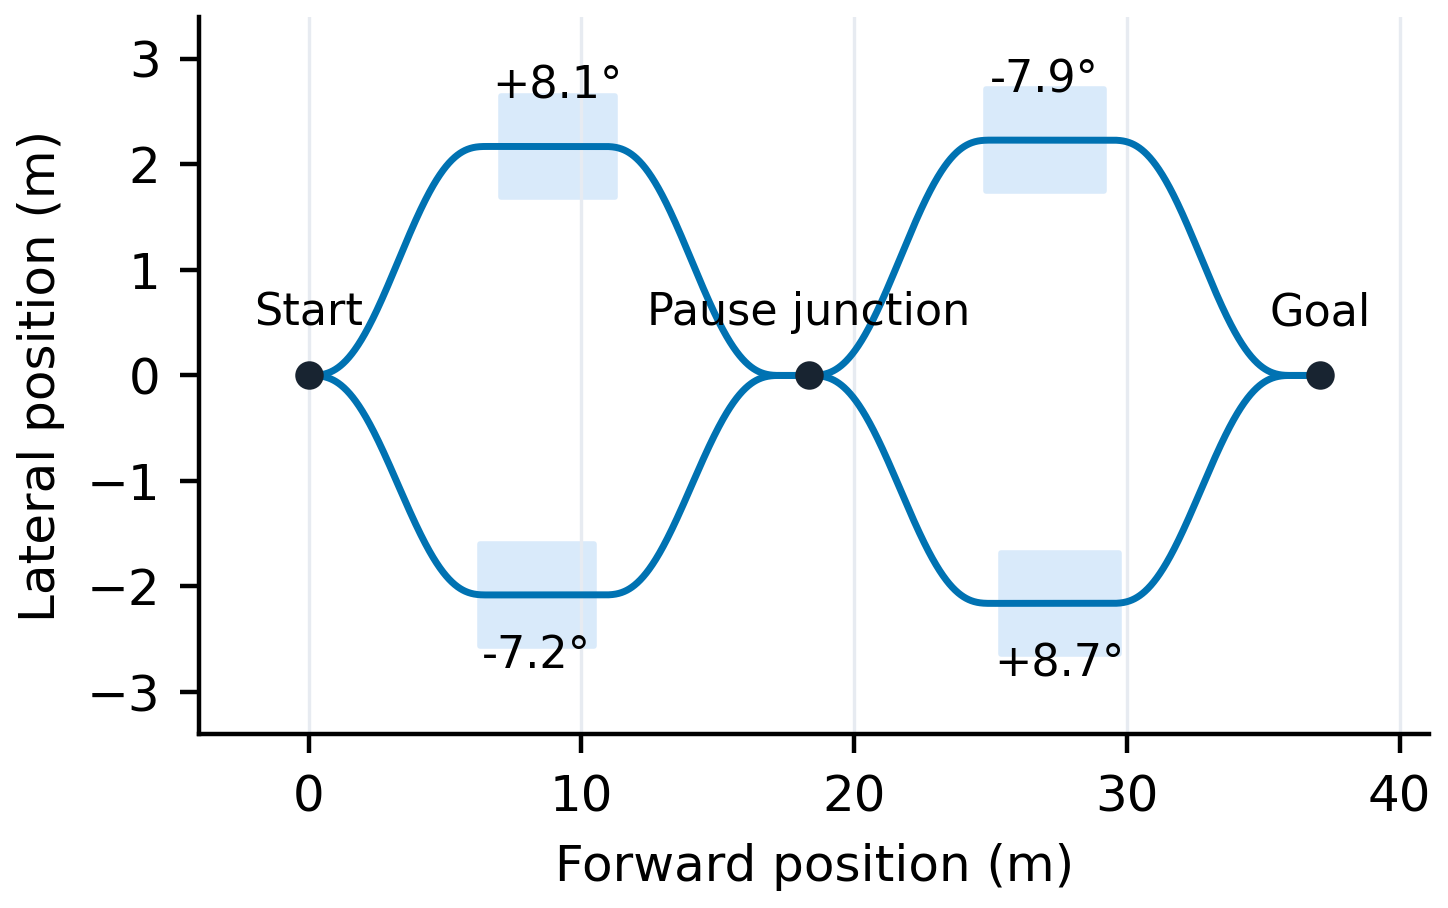
\includegraphics[width=\columnwidth]{figures/two_stage_course.png}
\caption{Top view of the shallow alternating-bank course used in the 12-course benchmark. The centerlines meet at a shared flat junction. Shading marks the nominal bank sections. The optional pause occurs at the shared junction.}
\label{fig:graph}
\end{figure}

Fig.~\ref{fig:graph} illustrates a course. Each stage has smooth approach and exit curves connecting the common landings to its two offset centerlines. The bank profile fades in and out along each branch. We varied the approach and exit length, bank length, lateral offset, bank angle, and longitudinal bank shift. Each course used a fixed deadline shared across planners and warm starts. The course families refer to the angle signs in the terrain specification. An alternating course reverses each branch's sign on the second stage. A persistent course retains each sign. The third family has both branches set to the same sign in at least one stage. The signs describe geometry. Motor heating comes from the crawler dynamics.

\subsection{Hexapod And Physics Execution}

The simulation used MuJoCo 3.9.0 \cite{todorov2012}. The hexapod had a floating chassis and three torque-actuated joints per leg at the coxa, femur and tibia. The simplified geometry was informed by the computer-aided design (CAD) assembly and had a modeled total mass of 82 kg, including the feet. From proximal to distal, the segment lengths were 0.157, 0.550, and 0.740 m, and the nominal joint torque limits were 90, 150, and 130 $\mathrm{N}{\cdot}\mathrm{m}$. A 3 s crawl gait generated foot targets from the branch centerline and simulated terrain height. Joint position and velocity feedback generated tracking torque. For supporting feet, a regularized least-squares allocation distributed the desired chassis force and moment. The physics step was 2 ms. The simulator recorded body position and contact counts and updated the thermal model every 20 ms using the root-mean-square applied actuator torque from that interval. Each walk began with a 2 s stand.

The 3 s gait staggers foot phases by 0.50 s. Each foot swings for 13.5\% of a cycle with a 0.09 m lift at mid-swing. The controller sets touchdown from the centerline pose and terrain height ahead of the body. When at least three feet meet the stance-support test, the force allocator distributes the commanded six-dimensional body wrench across them. For its unconstrained step, with support matrix $\mathbf{A}$ and body wrench $\mathbf{w}$, the allocated forces are
\begin{equation}
\mathbf{f}=\mathbf{A}^{\mathsf T}
   \left(\mathbf{A}\mathbf{A}^{\mathsf T}
    +0.02\mathbf{I}\right)^{-1}\mathbf{w}.
\end{equation}
We clamp vertical forces to be nonnegative and horizontal magnitudes at 0.65 times vertical force. The foot Jacobians map ground-reaction forces to joint torque terms. The resulting torques, combined with joint feedback, are clipped at the motor torque limits before stepping physics.

The earlier benchmark used 12 constructed heightfields at a target grid spacing of 0.12 m, four per family. The goal was 37.08 to 40.35 m forward from the start, with deadlines of 342 to 373 s. Arrival required the chassis to enter a 0.55 m radius around the goal. We checked lateral error against the selected centerline at the same forward coordinate and used a maximum error of 0.85 m. The thermal update and stop check precede the goal check within each 20 ms sample. Both the initial stand and the crawl count toward the deadline.

\subsection{Thermal Dynamics And Warm Starts}

The simulator tracks one temperature for each motor and updates the 18 states independently. For a 20 ms sample containing $n=10$ physics steps, the actuator root-mean-square torque is
\begin{equation}
q_i=\left(\frac{1}{n}\sum_{j=1}^n M_{ij}^2\right)^{1/2},
\end{equation}
where $M_{ij}$ is the applied actuator torque at physics step $j$. The thermal model uses the equilibrium $T_{i,\mathrm{eq}}$ for squared torque $q_i^2$ and updates the temperature over each interval $\Delta t$.

\begin{equation}
T_{i,\mathrm{eq}} = T_{\mathrm{amb}} + R\left(\frac{q_i}{q_{\mathrm{ref}}}\right)^2 ,
\label{eq:equilibrium}
\end{equation}

\begin{equation}
T_i(t+\Delta t) = T_{i,\mathrm{eq}} +
\bigl[T_i(t)-T_{i,\mathrm{eq}}\bigr]\exp(-\Delta t/\tau).
\label{eq:thermal-update}
\end{equation}

Ambient temperature $T_{\mathrm{amb}}$ was 25 \ensuremath{{}^{\circ}\mathrm{C}} and reference torque $q_{\mathrm{ref}}$ was 55 N\ensuremath{\cdot}m. The two 72-start benchmarks used the settings in Table~\ref{tab:settings}. All had a cooling time constant $\tau$ of 120 s. The parameter $R$ is the modeled equilibrium rise above ambient at the reference torque. For relative heating multiplier $m$, the configured settings give $R=72m\,{}^\circ\mathrm{C}$.

\begin{table}[!t]
\caption{Thermal settings and initial temperatures}
\label{tab:settings}
\centering
\footnotesize
\setlength{\tabcolsep}{4pt}
\renewcommand{\arraystretch}{1.18}
\begin{tabular}{@{}cccc@{}}
\hline
\shortstack{Heating\\multiplier} & \shortstack{Reference rise\\(\ensuremath{{}^{\circ}\mathrm{C}})} & \shortstack{Warm side\\(\ensuremath{{}^{\circ}\mathrm{C}})} & \shortstack{Cool side\\(\ensuremath{{}^{\circ}\mathrm{C}})} \\
\hline
0.46 & 33.12 & 67 & 45 \\
0.44 & 31.68 & 67 & 45 \\
0.45 & 32.40 & 68 & 48 \\
\hline
\end{tabular}
\end{table}


Each course used both warm-side assignments at each of the three thermal settings in Table~\ref{tab:settings}. All nine motors on one side started at the warm setting and all nine on the other side at the cool setting. Switching the warm side preserved the mean and maximum starting temperatures. Both planners received the same 18 starting temperatures for each scenario.

All controllers shared the same actuator torque derating. For a motor at temperature $T_i$, its nominal cap is multiplied by $1-0.25\,\operatorname{clip}((T_i-67)/3,0,1)$, with temperature in degrees Celsius. During a pause the forward speed command is zero and the stepping cycle continues. The physics replay leaves the chassis free to move under contact forces.

\subsection{Branch Profiles And Route Forecast}

We profiled each branch offline in separate nominal physics simulations at 65\% and 100\% of the 0.12 m/s nominal speed, with thermal derating disabled. We grouped samples after the stand by forward coordinate into equal-width bins of width $\Delta x$ close to 0.30 m. For a bin populated by $n_b$ samples, the forward-rate estimate is $\Delta x/(0.02 n_b)$ in meters per second. Motor load is the mean of the $n_b$ squared RMS torque samples. The two stand traces remain separate and initialize the forecast for the selected first command. The final bin also supplies the short flat approach from the nominal profile's stop point to the intermediate junction.

For a speed command $u$ expressed as a fraction of nominal speed, the forecast uses $\alpha=(u-0.65)/0.35$ to interpolate the forward rate $v_b$ and squared motor loads $\mathbf{L}_b$ in the current branch bin.
\begin{align}
 v_b(\alpha)&=(1-\alpha)v_{b,\mathrm{slow}}+\alpha v_{b,\mathrm{fast}},\\
 \mathbf{L}_b(\alpha)&=(1-\alpha)\mathbf{L}_{b,\mathrm{slow}}
                        +\alpha\mathbf{L}_{b,\mathrm{fast}} .
\end{align}
The forecast advances progress and Eq.~\eqref{eq:thermal-update} at 0.50 s intervals. Its forward goal approximation is $x_G-0.55$ m. The last forecast increment is clipped to that point. Nominal profiles use unmodified torque limits. Warm replays apply temperature-dependent torque clipping and carry the locomotion state across the junction.

\subsection{Forecasting The Load-Bearing Pause}

The forecast holds longitudinal position fixed during the pause and applies a constant equivalent squared torque for each motor. The relevant speed controller continues to update. For each of eight recorded 12 s pause windows on one development approach, four per approach speed, we used the simulated entry and exit temperatures, $T_{i,\mathrm{in}}$ and $T_{i,\mathrm{out}}$, to estimate the constant squared torque $q_{i,\mathrm{hold}}^2$ for a pause of duration $d$.

\begin{equation}
q_{i,\mathrm{hold}}^2 =
\frac{q_{\mathrm{ref}}^2}{R}
\left[T_{i,\mathrm{in}}-T_{\mathrm{amb}}+
\frac{T_{i,\mathrm{out}}-T_{i,\mathrm{in}}}{1-\exp(-d/\tau)}\right].
\end{equation}

We averaged inferred squared torques within each first-stage command and then averaged the two commands equally. Paused forecasts in both 72-start benchmarks used the same fitted loads (Table~\ref{tab:hold-loads}). Equation~\eqref{eq:thermal-update} predicts cooling for a motor when its junction-entry temperature exceeds the equilibrium implied by the hold load. At pause exit, the forecast resumes progress with the evolved temperature vector and current speed state. It evaluates the cutoff over the entire prediction, including the initial stand and the pause.

\begin{table}[!t]
\caption{Fitted squared torque during a 12 s hold in $(\mathrm{N}{\cdot}\mathrm{m})^2$}
\label{tab:hold-loads}
\centering
\footnotesize
\renewcommand{\arraystretch}{1.12}
\begin{tabular}{@{}lrrr@{}}
\hline
Leg & Coxa & Femur & Tibia \\
\hline
Left front & 5.943 & 2904.157 & 28.293 \\
Left middle & 3.320 & 3758.819 & 34.013 \\
Left rear & 1.669 & 2809.037 & 27.238 \\
Right front & 2.627 & 3030.600 & 29.827 \\
Right middle & 1.695 & 3578.708 & 34.374 \\
Right rear & 2.913 & 2911.345 & 29.891 \\
\hline
\end{tabular}
\end{table}

\subsection{Adapted Thermal Speed Controller}

Trujillo and Cutkosky \cite[Sec.~III-D, Eq.~(8)]{trujillo2009} used measured motor case temperature and a winding temperature limit to bound average heating over the upcoming gait period. At each footfall they inverted an empirical heating-versus-speed curve for the four-legged RiSE climber. We apply the fastest-feasible-speed rule to the 18 simulated motors using the first-order model in Eq.~\eqref{eq:thermal-update} and the hexapod's position-dependent branch profiles.

The adapted controller uses a 3 s gait period $g$. For a motor at its current temperature $T_i$, the controller uses the squared-torque budget $B_i$ obtained from Eq.~\eqref{eq:thermal-update} at $T_i(t+g)=T_{\mathrm{cap}}$.
\begin{equation}
B_i = \frac{q_{\mathrm{ref}}^2}{R}
    \left[T_i-T_{\mathrm{amb}}
      +\frac{T_{\mathrm{cap}}-T_i}{1-\exp(-g/\tau)}\right].
\label{eq:squared-torque-budget}
\end{equation}
Every 0.50 s, the regulator selects the largest $\alpha\in[0,1]$ satisfying
\begin{equation}
L_{b,i,\mathrm{slow}}+\alpha
  (L_{b,i,\mathrm{fast}}-L_{b,i,\mathrm{slow}})\leq B_i
  \quad\text{for all }i .
\label{eq:speed-constraints}
\end{equation}
If the intersection of all motor bounds is empty, the implementation records an infeasible update and commands the 65\% endpoint. The common torque derating and 70 \ensuremath{{}^{\circ}\mathrm{C}} stop remain active during physics execution. Both arms of the matched experiment used this controller.


\subsection{Matched Comparison Protocol}
\label{sec:matched-methods}

Both planners evaluate the supported routes without a pause using the adapted speed controller. The optional planner also evaluates each supported route with a 12\,s pause. For candidates that satisfy the temperature and deadline checks, both planners rank by earliest forecast arrival, then by lower forecast peak, then by route identifier. A tie on the same route favors zero pause. Both planners have a 2\,s online budget. The optional planner uses that same budget for forecasts at both durations.

The matched experiment used 12 courses distinct from those in the earlier benchmark. Each of the three terrain families contributed four courses. The projected length ranged from 37.44 to 40.29 m. We set each deadline by dividing that length by $0.108~\mathrm{m/s}$ and rounding to a whole second. The rate of 0.108 m/s is the median of the ratios of projected length to deadline in the first benchmark, rounded to three decimals. We fixed course geometries and deadlines before running the new profiles and used three thermal settings and two warm-side assignments on every course, for 72 paired starting scenarios. We collected 96 nominal branch profiles, one at each reference speed per branch. The same route had to be supported in both arms, so a branch was eligible only if both nominal runs completed. The adapted governor and thermal settings matched those in the supplementary controller comparison.

All zero-pause candidates use the exact forecast and physics callback of the original speed governor. A paused forecast uses the same progress step and governor update clock. Once the first junction is reached, it holds predicted longitudinal position for 24 forecast steps and applies the development hold loads in Table~\ref{tab:hold-loads}. The 0.50 s governor clock keeps advancing. During physics replay the gait also keeps cycling, with a zero forward command applied for 12 s. We recorded simulated chassis displacement and the forecast and simulated temperatures at pause entry and exit.

The primary outcome was goal completion within the deadline without a thermal stop. We also counted thermal stops as a separate outcome. Both rates use all 72 starting scenarios as the denominator, including those for which the planner rejected every route. The evaluation criterion set before the test was a gain of at least 10 percentage points with zero additional thermal stops. We also counted admissions, deadline misses, and junction reaches. We distinguished starts with an admissible paused forecast from starts selected for a pause. For every selected paused route, we also replayed the same route on the same warm start with zero pause. We compared the recorded trajectories up to the pause. The diagnostic replays were outside the control planner's outcome counts. Identical schedules selected by both planners on the same start shared one replay.

\section{Results}

\subsection{Goal Completion And Thermal Stops}

The optional-pause arm completed 29 of 72 starts, compared with 25 for the governor alone (Table~\ref{tab:matched-outcomes}). The four extra finishes yielded a gain of 5.6 percentage points. Each gain occurred on a different course in the alternating or same-sign-stage family (Fig.~\ref{fig:matched}). The same 25 starts finished under both planners. All four occurred in the 0.44 relative-heating setting. The robot reached the junction and paused for the full 12 s in all six selected scenarios. Two of the new admissions crossed the thermal limit after restarting, increasing the thermal-stop count from two to four. Both were left-warm starts in the setting with 68 \ensuremath{{}^{\circ}\mathrm{C}} initial warm motors. The results fall below the practical completion target and exceed the allowed additional stop count.

\begin{table}[!t]
\caption{Matched experiment outcomes across 72 starting scenarios}
\label{tab:matched-outcomes}
\centering
\footnotesize
\renewcommand{\arraystretch}{1.12}
\begin{tabular}{@{}lrr@{}}
\hline
Outcome & Governor only & Pause available \\
\hline
Completion & 25 & 29 \\
No route admitted & 45 & 39 \\
Thermal stop & 2 & 4 \\
Deadline, timeout, or other failure & 0 & 0 \\
\hline
\end{tabular}
\end{table}

\begin{figure*}[!t]
\centering
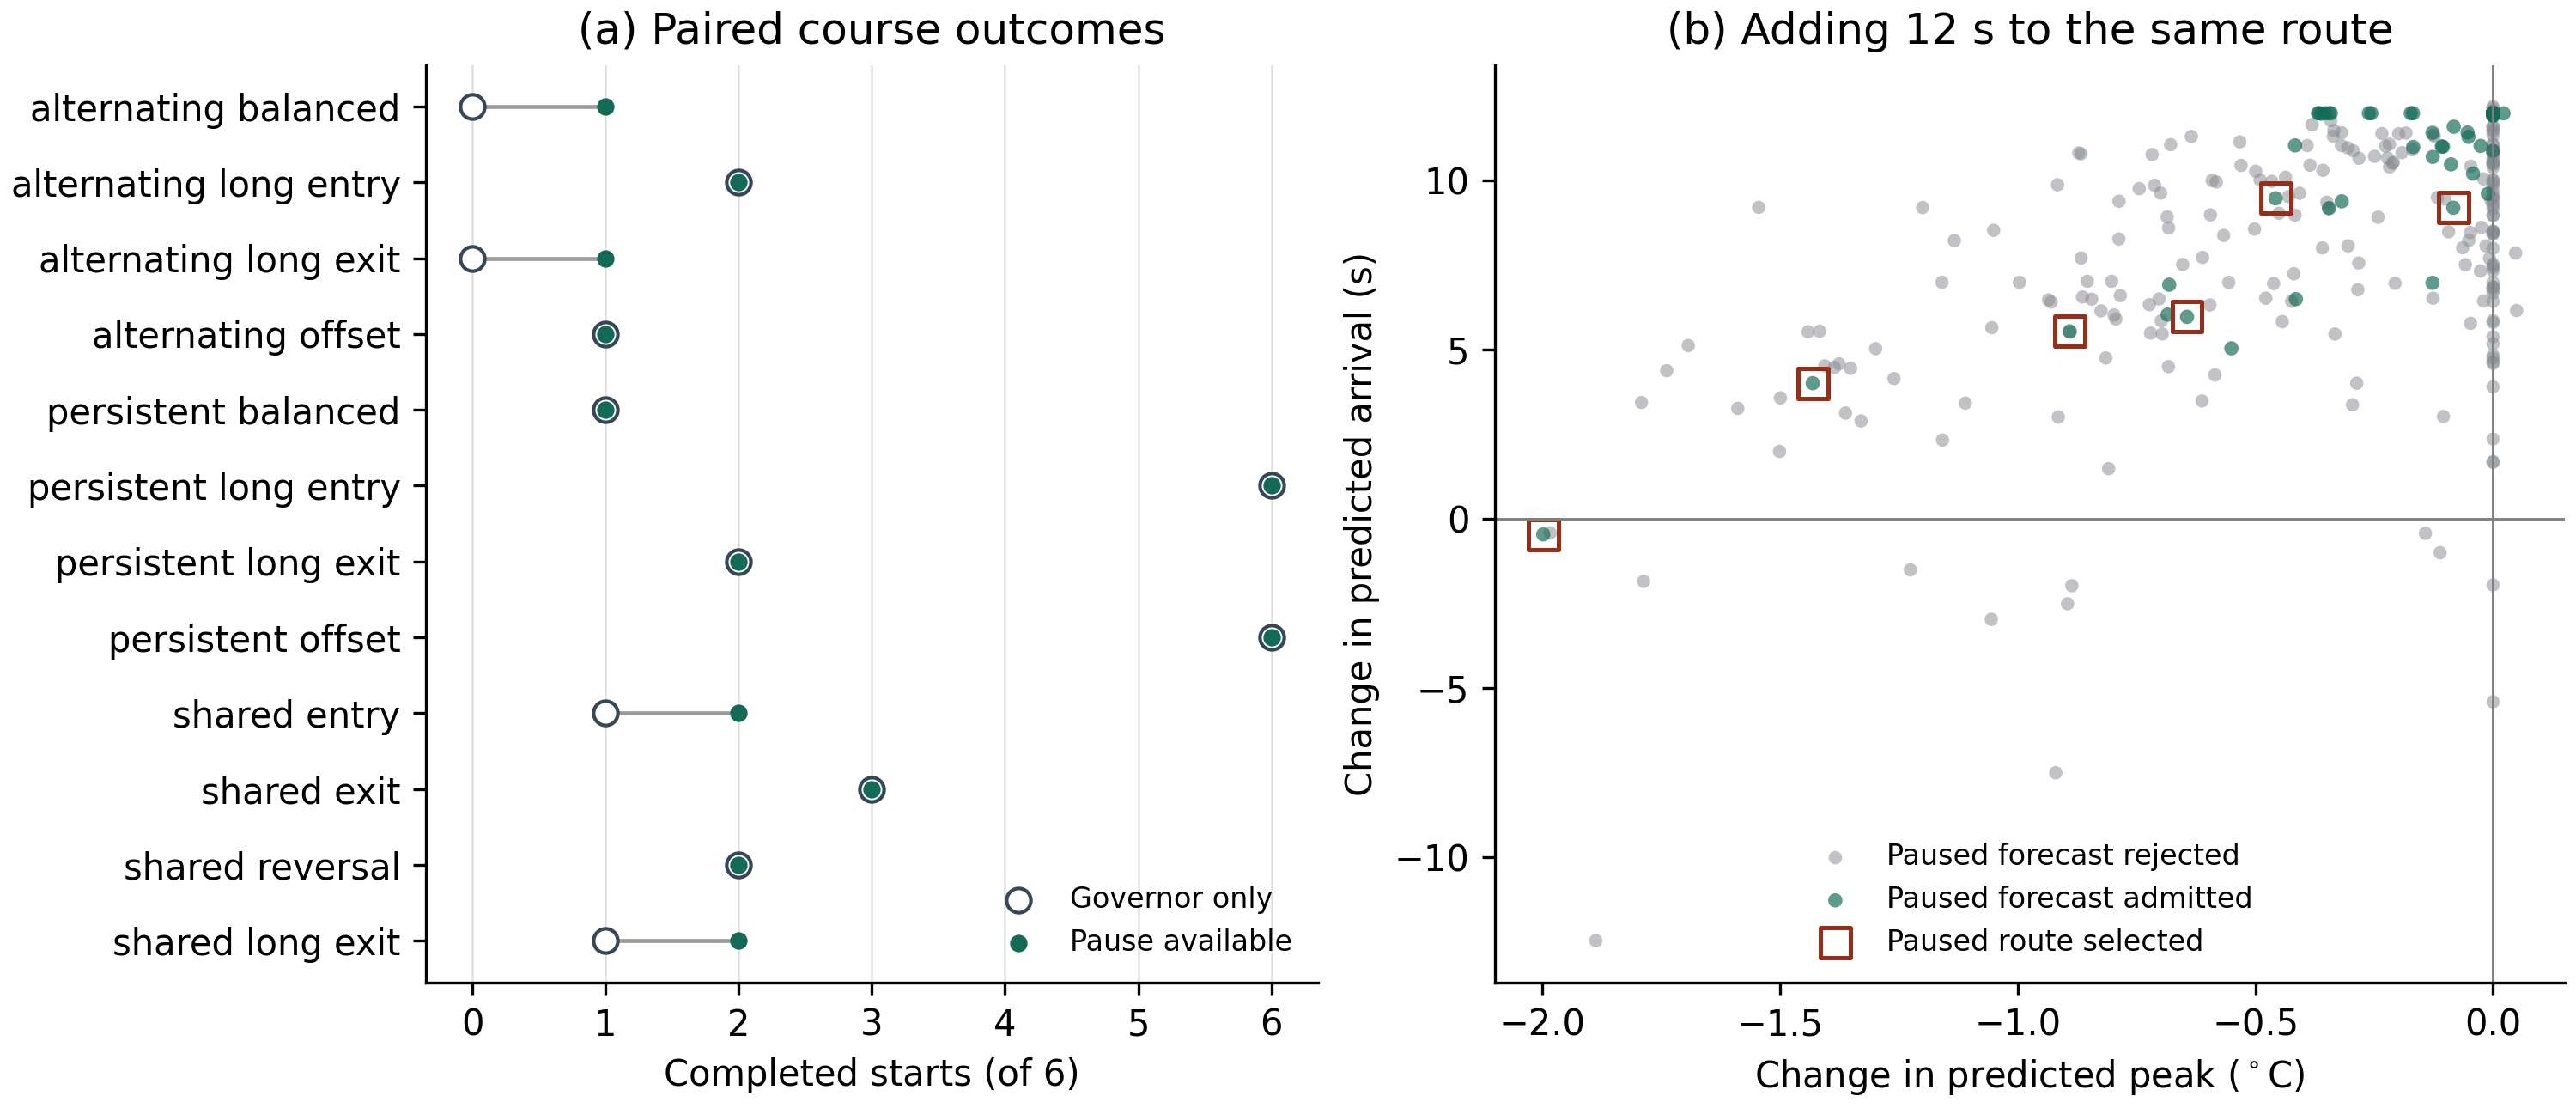
\includegraphics[width=.98\textwidth]{figures/matched_pause_outcomes.png}
\caption{Matched experiment on 12 new courses. Panel (a) gives the number of completed starts per course. Panel (b) shows the forecast change from adding a 12 s pause to the same route for each of the 288 route-and-start pairs. Negative peak changes indicate a cooler mission forecast. Six paused plans were selected.}
\label{fig:matched}
\end{figure*}

Table~\ref{tab:matched-courses} gives the course-level counts and the deadlines used by both arms. On the 24 starts in the 0.44 heating setting, the option raised completion from 15 to 19 with two stops in both arms. In the 0.45 setting, both arms finished five starts, and the option added two thermal stops. In the 0.46 setting, both arms finished five starts with zero thermal stops.

\begin{table*}[!t]
\caption{Geometry, deadlines and outcomes on the 12 matched-governor courses}
\label{tab:matched-courses}
\centering
\footnotesize
\setlength{\tabcolsep}{7pt}
\renewcommand{\arraystretch}{1.12}
\begin{tabular}{@{}lrrcccccc@{}}
\hline
& & & \multicolumn{3}{c}{Governor only} & \multicolumn{3}{c}{Pause available} \\
Course variant & Projected length (m) & Deadline (s) & Finished & Stopped & Rejected & Finished & Stopped & Rejected \\
\hline
Alternating balanced & 37.44 & 347 & 0 & 1 & 5 & 1 & 1 & 4 \\
Alternating long entry & 38.78 & 359 & 2 & 0 & 4 & 2 & 0 & 4 \\
Alternating long exit & 39.97 & 370 & 0 & 1 & 5 & 1 & 2 & 3 \\
Alternating offset & 38.50 & 356 & 1 & 0 & 5 & 1 & 0 & 5 \\
Persistent balanced & 37.48 & 347 & 1 & 0 & 5 & 1 & 0 & 5 \\
Persistent long entry & 39.42 & 365 & 6 & 0 & 0 & 6 & 0 & 0 \\
Persistent long exit & 39.64 & 367 & 2 & 0 & 4 & 2 & 0 & 4 \\
Persistent offset & 38.78 & 359 & 6 & 0 & 0 & 6 & 0 & 0 \\
Shared entry & 37.52 & 347 & 1 & 0 & 5 & 2 & 1 & 3 \\
Shared exit & 38.86 & 360 & 3 & 0 & 3 & 3 & 0 & 3 \\
Shared reversal & 39.35 & 364 & 2 & 0 & 4 & 2 & 0 & 4 \\
Shared long exit & 40.29 & 373 & 1 & 0 & 5 & 2 & 0 & 4 \\
\hline
\multicolumn{3}{@{}l}{Total across 72 starts} & 25 & 2 & 45 & 29 & 4 & 39 \\
\hline
\end{tabular}

\smallskip
\parbox{.96\textwidth}{Each course contributed six starts per arm. Stopped denotes a simulated thermal stop. Rejected denotes a start with no admitted route.}
\end{table*}

\subsection{Paired Replays On The Same Route}

Table~\ref{tab:matched-same-route} compares the six selected pauses with their zero-pause replays on the same routes and starts. Each pair used the same course, route, starting temperatures, and speed controller. The recorded trajectories matched through the last complete sample before the pause. The hottest motor at pause entry was a front femur in all six runs. It cooled by 1.01--1.44 \ensuremath{{}^{\circ}\mathrm{C}} during the hold. Maximum planar displacement during the pause ranged from 3.5 to 12.0 cm. The pause converted three thermal stops into finishes. One additional route completed at both durations, and its zero-pause forecast failed the planning cutoff. Two routes overheated at both durations. The four additional completions therefore comprise three routes that finished only with the pause and one route that also finished in its diagnostic run without a pause.

In the two paused replays that overheated, the motor cooled during the pause and reached the thermal limit after walking resumed. The temperatures recorded at the thermal stops exceeded the corresponding full-route forecast peaks by about 0.52 and 0.62 \ensuremath{{}^{\circ}\mathrm{C}}.

\begin{table*}[!t]
\caption{Fixed-route diagnostic for the six selected pauses}
\label{tab:matched-same-route}
\centering
\footnotesize
\renewcommand{\arraystretch}{1.12}
\begin{tabular}{@{}llrrrrll@{}}
\hline
& & \multicolumn{2}{c}{Forecast peak (\ensuremath{{}^{\circ}\mathrm{C}})}
  & \multicolumn{2}{c}{Observed peak (\ensuremath{{}^{\circ}\mathrm{C}})}
  & \multicolumn{2}{c}{Physics outcome} \\
Course & Start & 0 s & 12 s & 0 s & 12 s & 0 s & 12 s \\
\hline
Alternating balanced & 0.44 left & 69.553 & 69.096 & 70.014 & 69.304 & Thermal stop & Finish \\
Alternating long exit & 0.44 right & 70.377 & 69.486 & 70.001 & 69.663 & Thermal stop & Finish \\
Alternating long exit & 0.45 left & 70.914 & 69.483 & 70.009 & 70.000 & Thermal stop & Thermal stop \\
Shared entry & 0.44 right & 69.552 & 69.469 & 69.860 & 69.830 & Finish & Finish \\
Shared entry & 0.45 left & 71.376 & 69.378 & 70.009 & 70.001 & Thermal stop & Thermal stop \\
Shared long exit & 0.44 right & 70.136 & 69.492 & 70.011 & 69.962 & Thermal stop & Finish \\
\hline
\end{tabular}

\smallskip
\parbox{.96\textwidth}{Start gives relative heating and the initially warmer side. All zero-pause forecasts in this table failed the 69.50 \ensuremath{{}^{\circ}\mathrm{C}} gate. They were replayed as diagnostics and do not count as control-arm attempts. Observed peaks for thermal stops are limited by the first sample at or above 70 \ensuremath{{}^{\circ}\mathrm{C}}.}
\end{table*}

\subsection{Forecast Screening And Route Choice}

All 96 nominal traces completed, so every paired start had four supported geometric routes. The two arms produced 288 shared zero-pause forecasts and the optional arm produced 288 additional paused forecasts. All forecasts met their deadlines. The smallest forecast time to spare was 32.20 s, and all candidate rejections were due to the temperature cutoff.

Of the 288 route-and-start pairs, 40 qualified at both durations, 12 qualified only with the pause, and 236 failed at both durations. A paused option qualified on 33 starts. The planner selected a pause on six starts across four courses, all initially rejected by the zero-pause arm. It retained the same route and zero pause on the 27 originally admitted starts. Neither arm timed out. Their longest online planning times were 0.070 s and 0.128 s for the zero-pause and optional-pause arms respectively. With the same 27 unpaused selections in both arms, the six new admissions capped the achievable gain at 8.3 percentage points.

Fig.~\ref{fig:matched} shows both the course outcomes and the paired forecast changes. Across 288 route-and-start pairs, the pause reduced the forecast peak in 186 cases, left it unchanged in 99, and increased it in three. Adding the hold shifted the predicted arrival by a median of 9.25 s. The middle half of the changes ranged from 6.43 to 11.07 s. The forecast applies feedback speed commands after the hold. Thirteen route pairs had an earlier forecast arrival with a pause.

\section{Discussion}

The shared-entry course illustrates the effect of the forecast cutoff. The route without a pause had a forecast peak of 69.552 \ensuremath{{}^{\circ}\mathrm{C}}, above the 69.50 \ensuremath{{}^{\circ}\mathrm{C}} planning cutoff. The unpaused diagnostic walk finished with a peak of 69.860 \ensuremath{{}^{\circ}\mathrm{C}}, below the 70 \ensuremath{{}^{\circ}\mathrm{C}} execution limit. The additional finish on that course resulted from admitting the route under the paused forecast.

Across all six paused replays, the peak recorded up to completion or thermal stop exceeded the forecast peak by 0.18 to 0.62 \ensuremath{{}^{\circ}\mathrm{C}}. The paired traces show cooling during the pause followed by overheating on two routes after walking resumed. In the earlier benchmark, 28 of the 38 thermal stops under the time-only fallback occurred before the robot reached the pause location. Both sets of runs show why temperature screening covers the approach and the remaining walk.

\subsection{Simulation Scope And Verification}

Both benchmarks used synthetic two-stage courses, known starting motor temperatures, and the one-state actuator model in Eq.~\eqref{eq:thermal-update}. The matched forecasts passed the deadline check, so this benchmark compares the temperature screening and route choices under deadlines with forecast time to spare.

A verification pass recomputed the 576 forecasts and 144 planning decisions from the 96 branch profiles. Each recorded temperature series reproduced the thermal update from the applied motor torques. The 39 physics replays comprised 27 unpaused runs shared by the planners, six paused runs chosen by the optional planner, and six unpaused diagnostic replays. Each same-route pair agreed in torque, chassis position, foot-contact count, and motor temperature before the pause. The verified records contained 6,226 to 6,852 torque samples at 20 ms intervals per pair.

\section{Conclusion}

In 72 paired simulations, offering a 12\,s junction pause increased goal completions by 5.6 percentage points and added two overheating stops. Three of six selected routes changed from an overheating stop to a finish when the pause was applied on the same route. The planner fell short of the specified criterion of a 10-point improvement with zero additional thermal stops.

\appendices

\section{Development Trials}

In the initial 36-start comparison, a planner with labeled starting temperatures finished 32 missions and a planner averaging over two possible warm-side assignments finished 31. A supplemental bank-order comparison placed the same two stage geometries in opposite order and held the deadlines and initial temperature vectors fixed within each pair. The initial thermal settings produced no admissions. In a follow-up under simulated heating settings selected nearer the admission boundary, the labeled planner finished 13 of 24 starts and the anonymous planner finished seven. Reversing the stages changed completion for the labeled planner in three matched comparisons, all when the right-side motors were warm.

The first pause trial used one left-warm unequal-banks start for which all 16 original route-and-speed schedules overheated. We evaluated 6, 12, and 24 s pauses at the same junction. Eight of the 16 original walks stopped before the pause could trigger. Their outcomes carried over because the command up to the junction is identical. The other eight schedules received a continuous physics replay for each duration. Hottest motor temperature was lower after the pause in all 24 replays that held at the junction.

Fig.~\ref{fig:pilot} shows four replays of the same schedule. Its zero-pause control reproduced the original unpaused torque, body-position, contact-count, and temperature arrays. The 12 s pause cooled the hottest entry motor, the left front femur, from 66.75 to 65.79 \ensuremath{{}^{\circ}\mathrm{C}}. The body moved at most 6.83 cm from its pause-entry position. The mission finished in 350.32 s with a peak of 69.91 \ensuremath{{}^{\circ}\mathrm{C}} and a 352 s deadline. On the same schedule, a 6 s pause yielded a thermal stop at 325.16 s, while a 24 s pause stayed below the thermal limit through the deadline. Among the four tested durations on this schedule, only the 12 s pause finished by the deadline.

\begin{figure}[!t]
\centering
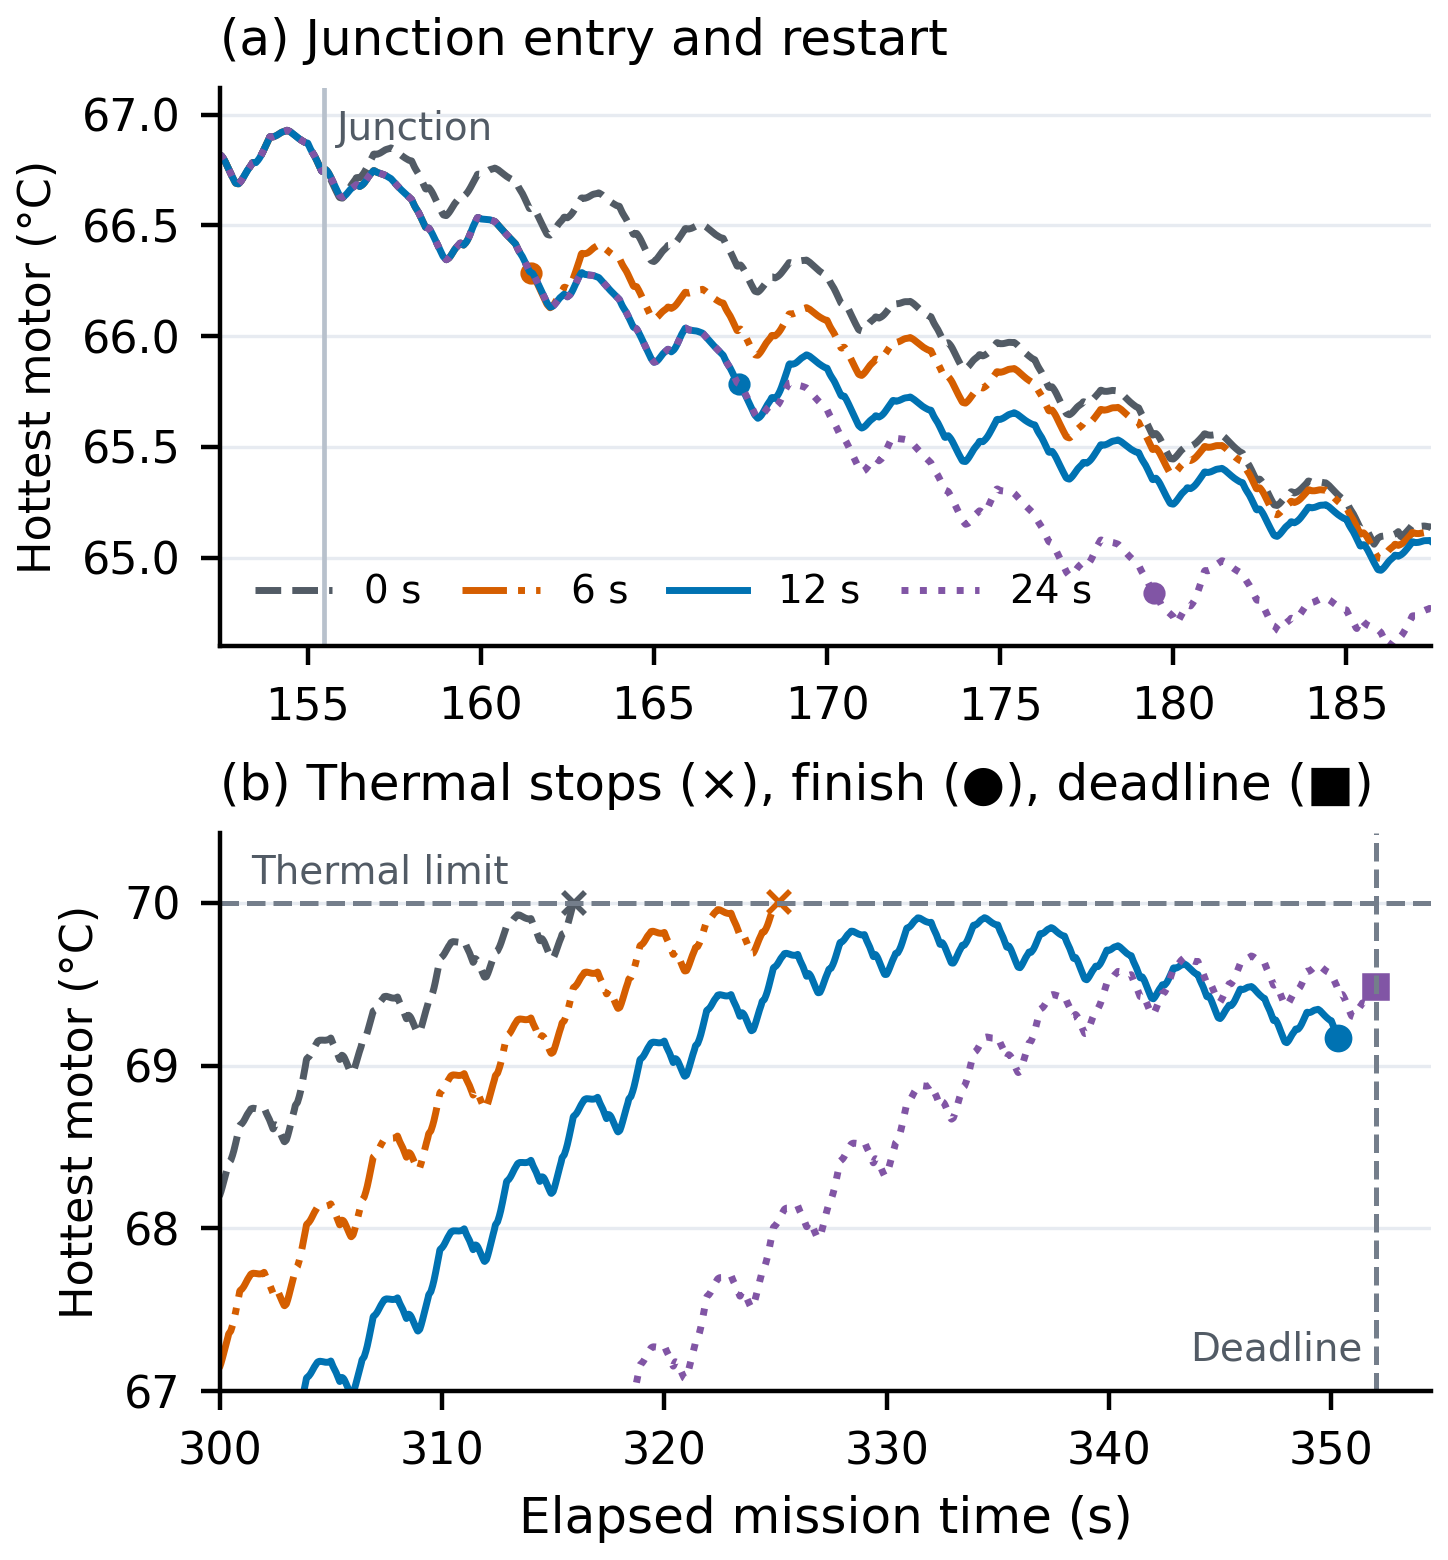
\includegraphics[width=\columnwidth]{figures/pause_pilot_durations.png}
\caption{Four durations on a single unequal-banks schedule. Curves show the hottest motor at each sample. The upper panel focuses on junction arrival and restart. The lower panel shows the mission outcomes. Each line ends at the first simulated stop or goal.}
\label{fig:pilot}
\end{figure}

Table~\ref{tab:pilot-outcomes} reports the outcomes for all 16 schedules at each tested duration. The counts at positive durations include the eight approach-stage stops. The 12 s test was the only duration with a finish.

\begin{table}[!t]
\caption{Outcomes by pause duration in the unequal-banks development trial}
\label{tab:pilot-outcomes}
\centering
\footnotesize
\renewcommand{\arraystretch}{1.11}
\begin{tabular}{@{}lrrr@{}}
\hline
Pause (s) & Finished & Thermal stop & Deadline miss \\
\hline
0 & 0 & 16 & 0 \\
6 & 0 & 15 & 1 \\
12 & 1 & 14 & 1 \\
24 & 0 & 14 & 2 \\
\hline
\end{tabular}
\end{table}

The four-course development comparison used the same selected schedules with and without a 12 s pause. A schedule was selected for 22 of 24 starts. Each matched pair agreed sample by sample up to the first junction, or for the entire trace if the junction was never reached. Completion rose from four to seven. All three new completions were on the crossed split, where the pause converted a thermal stop into a finish. All four control completions also finished with the pause. Six pairs overheated before reaching the junction. Among the 16 that reached it, the hottest motor cooled by 0.85 to 1.28 \ensuremath{{}^{\circ}\mathrm{C}} over the pause.

Table~\ref{tab:development-errors} reports the forecast errors on the 22 paired development cases. The full forecast starts at departure. The separate hold calculation starts from the simulated junction-entry temperatures. The full paused forecast rejected all 15 observed thermal stops and admitted four of the seven observed finishes at the inherited 69.50 \ensuremath{{}^{\circ}\mathrm{C}} cutoff. The three excluded finishes had forecasts of 69.60 to 69.87 \ensuremath{{}^{\circ}\mathrm{C}}. We retained the cutoff for the larger comparison.

\begin{table}[!t]
\caption{Forecast mean absolute errors on paused development walks}
\label{tab:development-errors}
\centering
\footnotesize
\setlength{\tabcolsep}{4pt}
\renewcommand{\arraystretch}{1.13}
\begin{tabularx}{\columnwidth}{@{}>{\raggedright\arraybackslash}Xrr@{}}
\hline
Statistic & Walks & Error \\
\hline
Mission peak, full forecast & 7 & 0.092 \ensuremath{{}^{\circ}\mathrm{C}} \\
Finish, full forecast & 7 & 1.56 s \\
Finish, nominal time plus 12 s & 7 & 1.75 s \\
Maximum at pause exit, full forecast & 16 & 0.195 \ensuremath{{}^{\circ}\mathrm{C}} \\
Pause-exit motor, simulated entry & 16 & 0.030 \ensuremath{{}^{\circ}\mathrm{C}} \\
\hline
\end{tabularx}
\end{table}

\section{Earlier Planner Comparisons}
\label{app:earlier-benchmark}

\subsection{Planner Rules}

A separate reactive speed rule used by the three frozen-benchmark planners ramps the speed cap toward 65\% over 2 s when the hottest motor reaches 67 \ensuremath{{}^{\circ}\mathrm{C}}, and begins restoring it at or below 65.50 \ensuremath{{}^{\circ}\mathrm{C}}. The forward command takes the lesser of planned speed and this cap. The planned speed commands were 65\% or 100\% of nominal speed, which gave 16 route and speed schedules per course. After junction crossing, the planned stage command changed at 0.5 of nominal speed per second. A pause set the forward speed command to zero while the crawl phase continued.

All three planners first searched the no-pause schedules. A candidate qualified if its predicted peak was strictly below 69.50 \ensuremath{{}^{\circ}\mathrm{C}} and its finish forecast was within the deadline. Among qualifying schedules, the planner chose the lowest predicted peak, then the earliest predicted finish and the schedule identifier. A fallback ran only on an original planning rejection and shared the same total two-second online budget. Offline nominal profiling was outside that budget. The planners used the same physics controller in execution. Table~\ref{tab:methods} summarizes their fallback rules.

\begin{table}[!t]
\caption{Fallback policies following rejection by the fixed planner}
\label{tab:methods}
\centering
\footnotesize
\setlength{\tabcolsep}{4pt}
\renewcommand{\arraystretch}{1.18}
\begin{tabularx}{\columnwidth}{@{}>{\raggedright\arraybackslash}p{.28\columnwidth}>{\raggedright\arraybackslash}X@{}}
\hline
Planner & Fallback after rejection \\
\hline
Fixed reactive & Record a planning rejection. \\
Time-only pause fallback & Add 12 s to the no-pause arrival forecast and filter by deadline. Rank by no-pause peak, predicted arrival, and schedule identifier. The fallback applies no thermal admission cutoff. \\
Per-motor pause forecast & Forecast the complete paused schedule, screen with the same 69.50 \ensuremath{{}^{\circ}\mathrm{C}} cutoff and deadline, then rank qualifying schedules by predicted peak and finish time. \\
\hline
\end{tabularx}
\end{table}


All methods required complete nominal profiles at both speeds for each candidate branch. The geometry and deadlines were set before nominal profiling and warm replay. A selected schedule was tested by one continuous physics replay. Methods that selected identical schedules on the same start shared the same deterministic trace, with the pause duration included in the schedule identity.

The practical criterion set before this benchmark was a gain of at least 10 percentage points with no additional observed thermal stops. Completion rates use all 72 starting scenarios as the denominator.

We recomputed the complete paused forecasts for the 48 schedules selected after initial rejection by the time-only fallback. We applied cutoffs of 69.50 and 70.00 degrees Celsius to the same forecasts and counted admissions by the observed replay outcome. We also recorded the junction reachability of each stopped run.

\subsection{Outcomes On The Earlier 12 Courses}

Table~\ref{tab:course-outcomes} lists the earlier course lengths and deadlines. All 96 nominal branch profiles completed, retaining both branches at both speeds for every course. The three frozen planners generated 216 decisions on 72 paired starts and selected 72 distinct warm replays. A separate audit checked decision coverage, the inherited model and source lock, and every warm trace. The longest decision took 0.169 s against the 2 s budget. Table~\ref{tab:outcomes} and Fig.~\ref{fig:screening} include the frozen outcomes and the subsequent comparison with the adapted controller.

\begin{table}[!t]
\caption{Mission outcomes across 72 starts per planner}
\label{tab:outcomes}
\centering
\footnotesize
\setlength{\tabcolsep}{4pt}
\renewcommand{\arraystretch}{1.18}
\begin{tabular}{@{}lrrrr@{}}
\hline
Planner & \shortstack{Com-\\pleted} & \shortstack{Re-\\jected} & \shortstack{Thermal\\stop} & \shortstack{Deadline\\miss} \\
\hline
Fixed reactive & 18 & 50 & 0 & 4 \\
Time-only fallback & 28 & 2 & 38 & 4 \\
Per-motor forecast & 20 & 48 & 0 & 4 \\
Adapted speed rule & 30 & 39 & 3 & 0 \\
\hline
\end{tabular}
\end{table}


The per-motor fallback recovered two of the fixed planner's rejected starts and preserved its 18 finishes. The 2.8-percentage-point gain was below the prespecified 10-point target. Relative to the time-only fallback, the per-motor planner lost eight finishes and reduced thermal stops by 38. Its paired completion difference was $-11.1$ percentage points.

Table~\ref{tab:course-outcomes} shows concentration of the two gains on the shallow alternating-bank course. They occurred in the near-boundary setting, one for each initial warm-side assignment, where totals across all courses were 13 of 24 finishes for the pause forecaster and 11 of 24 for the fixed planner. The other settings yielded the same completion counts under both policies. For each recovered start, the chosen schedule used 65\% planned speed on the first stage and 100\% on the second.

\begin{table*}[!t]
\caption{Courses and completions out of six starts per planner per course}
\label{tab:course-outcomes}
\centering
\footnotesize
\setlength{\tabcolsep}{8pt}
\renewcommand{\arraystretch}{1.12}
\begin{tabular}{@{}llrrcccc@{}}
\hline
Family & Course variant & \shortstack{Goal $x$\\(m)} & \shortstack{Deadline\\(s)} &
\shortstack{Fixed\\reactive} & \shortstack{Time-only\\fallback} &
\shortstack{Per-motor\\forecast} & \shortstack{Adapted\\speed rule} \\
\hline
Alternating & Shallow & 37.08 & 342 & 0 & 2 & 2 & 0 \\
 & Early & 38.29 & 352 & 1 & 2 & 1 & 1 \\
 & Long second & 39.41 & 369 & 1 & 2 & 1 & 1 \\
 & Long first & 39.03 & 366 & 0 & 2 & 0 & 2 \\
\hline
Persistent & Shallow & 37.24 & 344 & 4 & 4 & 4 & 6 \\
 & Offset & 38.00 & 350 & 0 & 0 & 0 & 2 \\
 & Long second & 40.04 & 371 & 4 & 5 & 4 & 6 \\
 & Long first & 39.38 & 370 & 0 & 1 & 0 & 2 \\
\hline
Same-sign stage & First & 37.85 & 348 & 2 & 3 & 2 & 4 \\
 & Second & 38.77 & 356 & 1 & 1 & 1 & 1 \\
 & Reversal & 39.08 & 363 & 2 & 2 & 2 & 2 \\
 & Late long & 40.35 & 373 & 3 & 4 & 3 & 3 \\
\hline
\multicolumn{4}{@{}l}{Total across 72 starts} & 18 & 28 & 20 & 30 \\
\hline
\end{tabular}
\end{table*}

Fig.~\ref{fig:paths} shows the two additional finishes. Exchanging the warm side reversed the selected branch on each stage. The left-warm walk finished at 340.02 s with a peak of 68.96 \ensuremath{{}^{\circ}\mathrm{C}}. The right-warm walk finished at 341.44 s with a peak of 69.21 \ensuremath{{}^{\circ}\mathrm{C}}. Against the 342 s deadline, the observed time headroom was 1.98 and 0.56 s, respectively. These replays demonstrate both a switch in route choice and a completed mission following each mirrored choice.

\begin{figure*}[!t]
\centering
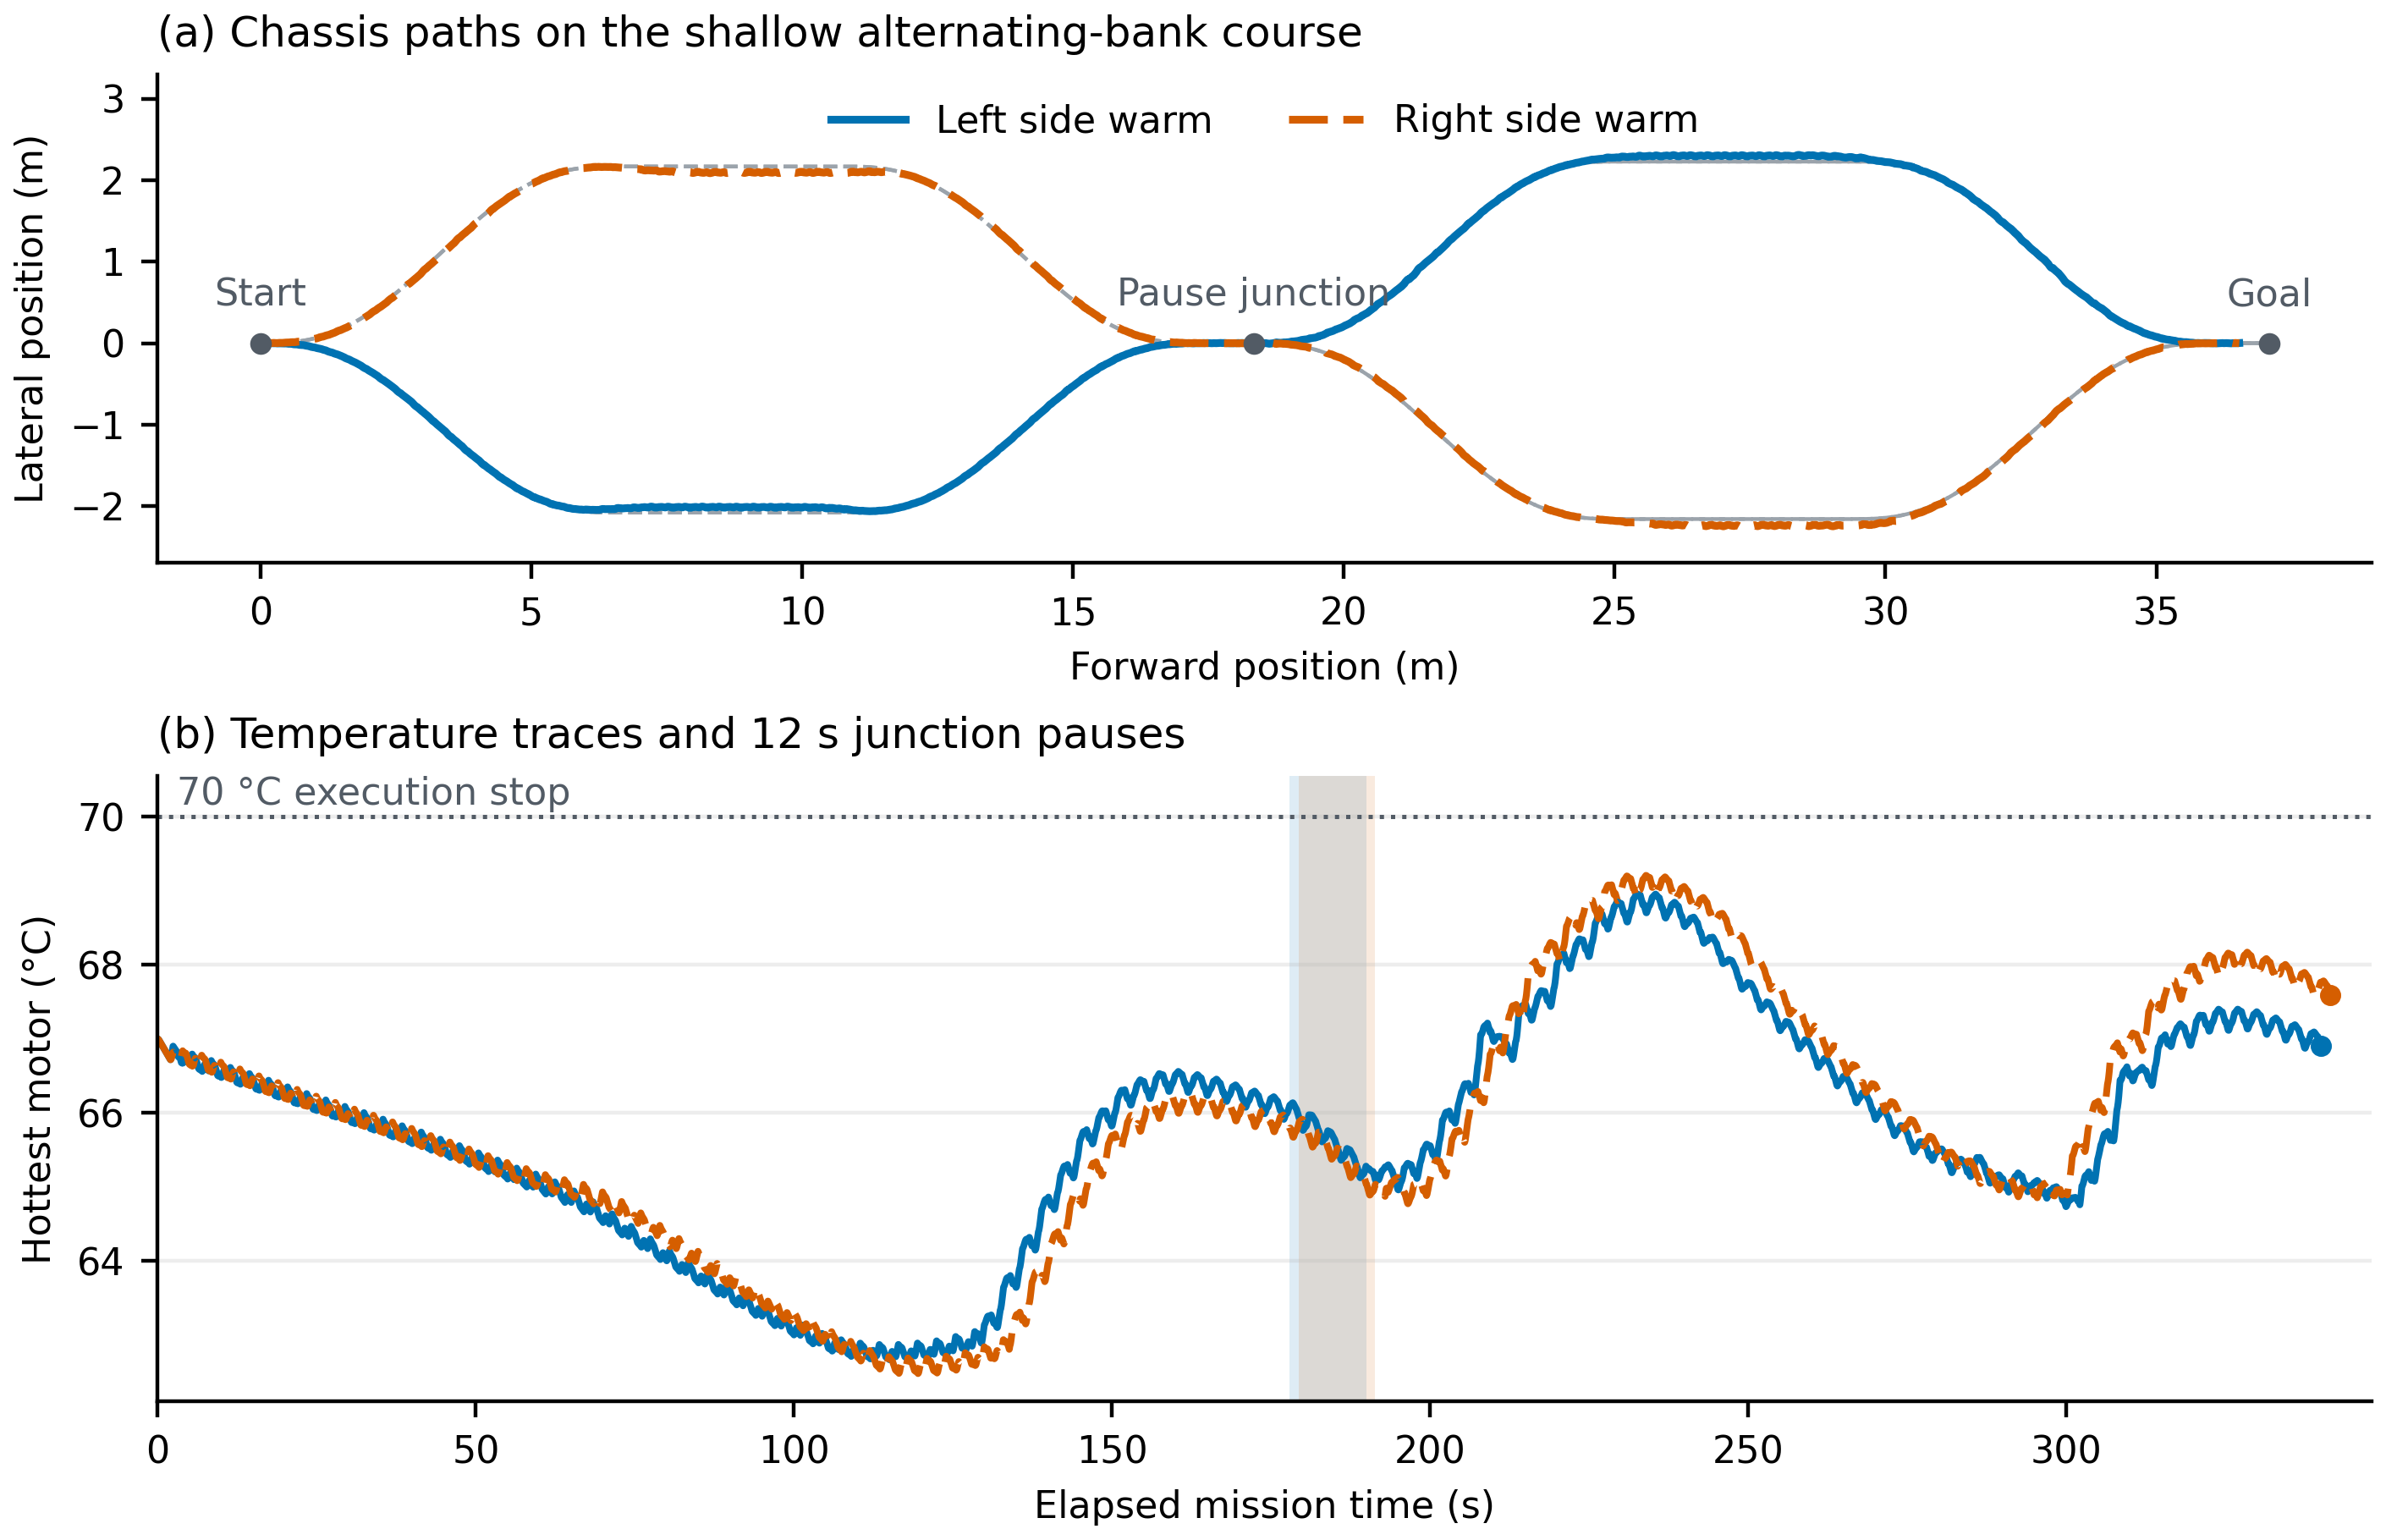
\includegraphics[width=.88\textwidth]{figures/junction_paths_and_temperatures.png}
\caption{Chassis position and maximum motor temperature for the two additional completions. The upper panel shows branch centerlines in gray and the simulated chassis traces in blue and orange. The lower panel marks each 12 s pause with a shade matching its trace. Dots at the ends mark mission completion.}
\label{fig:paths}
\end{figure*}

\begin{figure*}[!t]
\centering
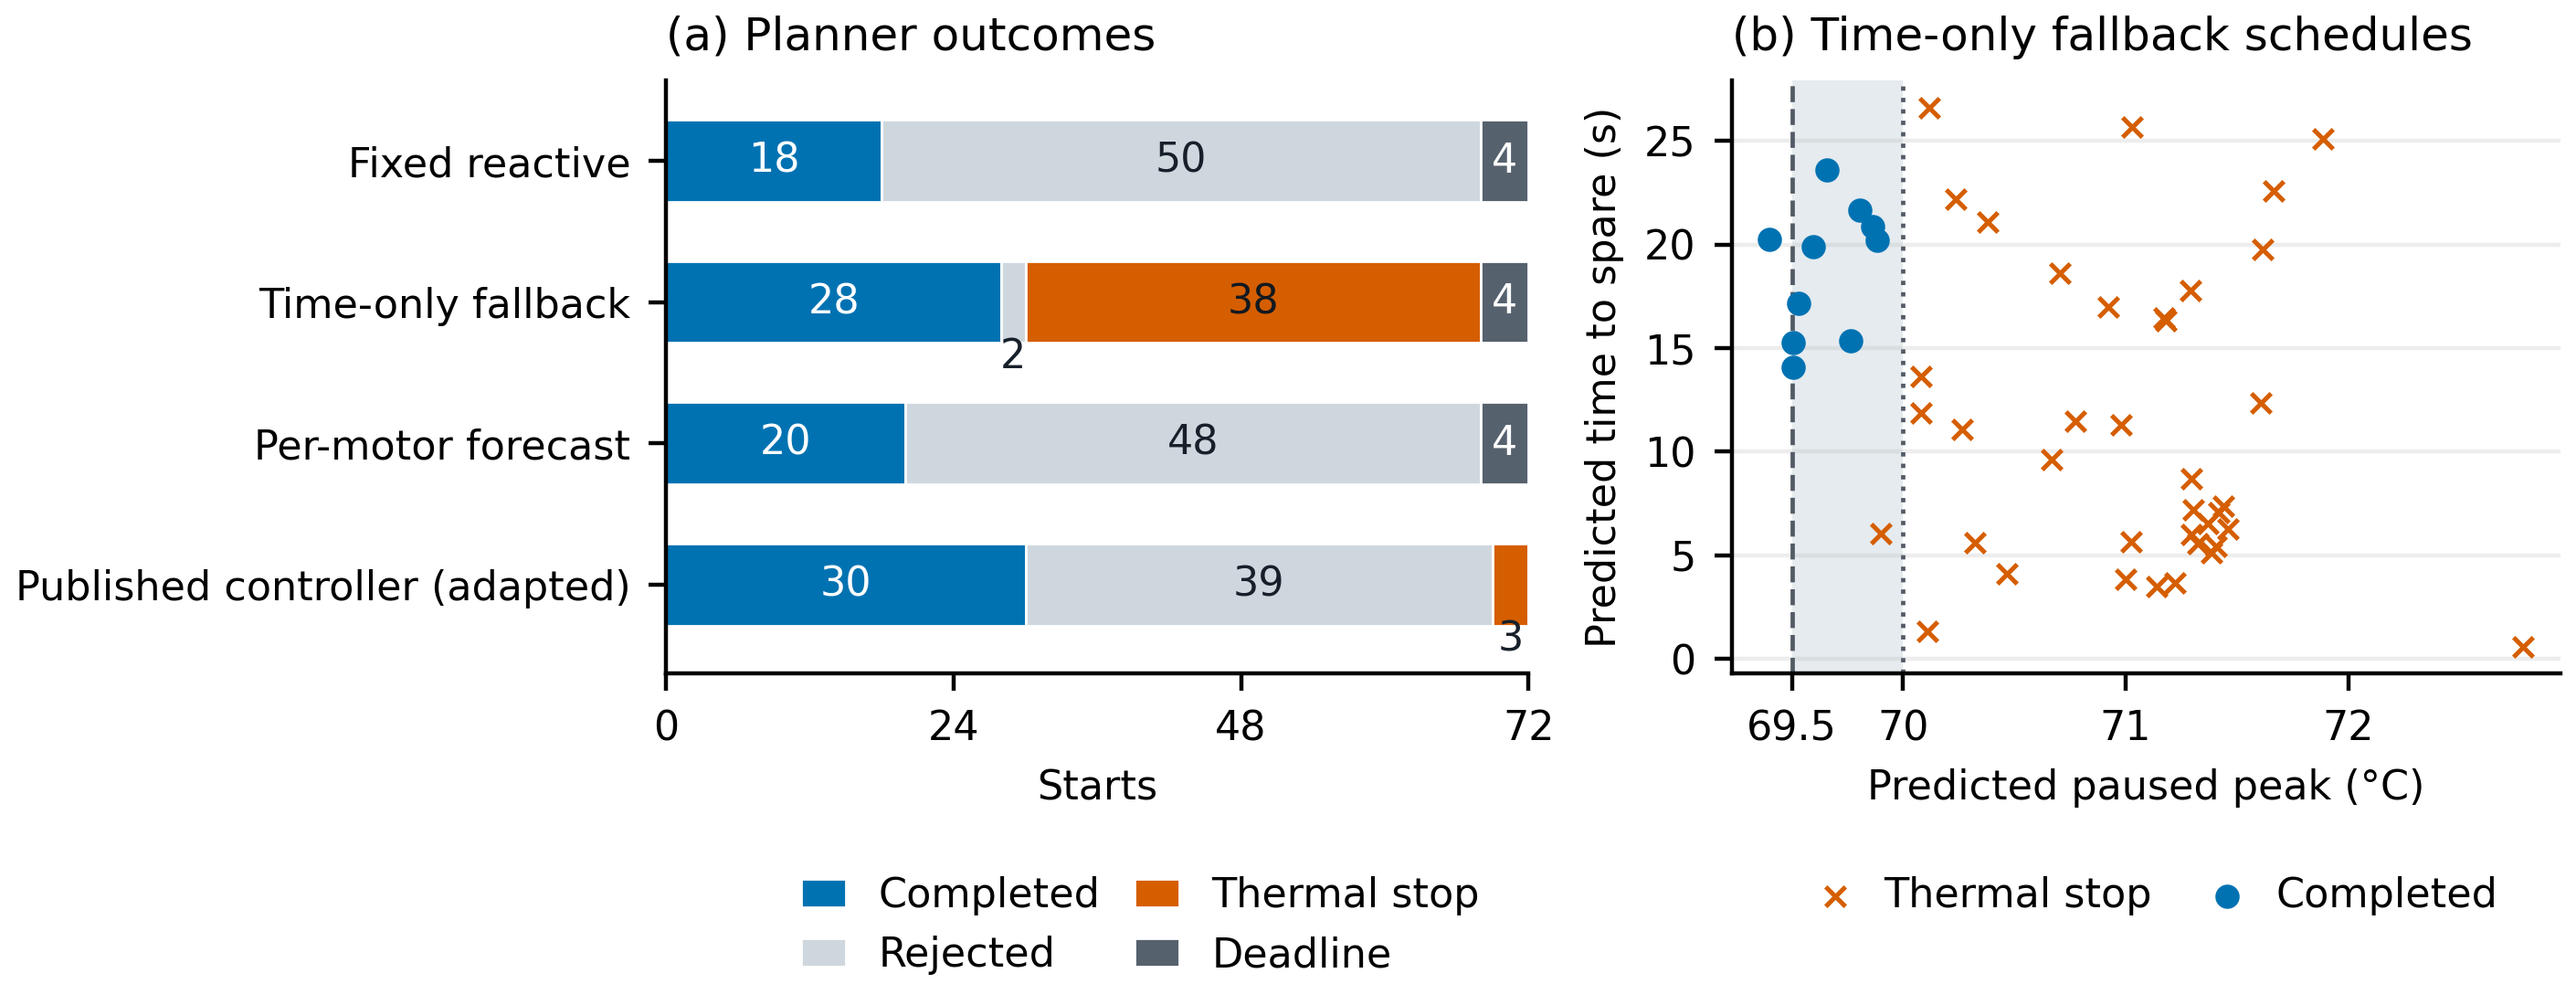
\includegraphics[width=.94\textwidth]{figures/benchmark_outcomes_and_screening.png}
\caption{Planner outcomes over 72 starts and the 48 attempted time-only pause schedules. The right panel shows plotted forecasts and observed outcomes. The shaded region spans the 69.50 \ensuremath{{}^{\circ}\mathrm{C}} planning cutoff (dashed) to the 70 \ensuremath{{}^{\circ}\mathrm{C}} execution stop (dotted).}
\label{fig:screening}
\end{figure*}

\subsection{Published-Controller Comparison}

The comparison applied the adapted speed controller after the earlier three-planner benchmark and reused the same 72 starting scenarios. The route selection evaluated the four routes with zero pause and applied the same ranking and cutoff as the matched controller arm. The control law and route ranking therefore both differ from those in the three-planner comparison.

The adapted speed rule finished 30 of 72 starts and recorded three thermal stops. It finished 14 starts missed by the pause forecaster, and the pause forecaster finished four missed by the adapted method. The net difference for the pause forecaster was $-13.9$ percentage points. Both shallow alternating-bank starts recovered by the pause forecaster reached the junction under the adapted rule and later overheated. The third thermal stop, on the early alternating-bank course, occurred before the junction. All 72 controller decisions stayed under budget (maximum 0.065 s). All 33 selected replays were audited against their traces.

\subsection{Fixed-Candidate Screening And Pause Reachability}
\label{sec:screen-diagnostic}

In the post hoc analysis, all 48 fixed time-only fallback candidates passed the complete forecast's time gate. At the 69.50 \ensuremath{{}^{\circ}\mathrm{C}} cutoff, the screen rejected 38 stopped walks and nine finishes. One finish passed the screen. The per-motor planner selected different paused schedules for its two additional completions. The time-only fallback also finished both starts. Table~\ref{tab:screen-counts} distinguishes the disposition of these individual schedules from completion rates for the planners.

The eight starts that only the time-only planner completed had forecasts from 69.504 to 69.882 \ensuremath{{}^{\circ}\mathrm{C}}. All eight finished within the simulated thermal limit and deadline and failed the 0.50 \ensuremath{{}^{\circ}\mathrm{C}} forecast margin. Applying the 70.00 \ensuremath{{}^{\circ}\mathrm{C}} cutoff to the same forecasts admitted ten finishes and one stopped walk.

\begin{table}[!t]
\caption{Post hoc screening of 48 fixed time-only fallback schedules}
\label{tab:screen-counts}
\centering
\footnotesize
\setlength{\tabcolsep}{5pt}
\renewcommand{\arraystretch}{1.15}
\begin{tabular}{@{}lrrrr@{}}
\hline
Forecast & \multicolumn{2}{c}{Observed finish} & \multicolumn{2}{c}{Observed stop} \\
cutoff & Admit & Reject & Admit & Reject \\
\hline
69.50 \ensuremath{{}^{\circ}\mathrm{C}} & 1 & 9 & 0 & 38 \\
70.00 \ensuremath{{}^{\circ}\mathrm{C}} & 10 & 0 & 1 & 37 \\
\hline
\end{tabular}
\end{table}

Of the 38 stops, 28 occurred before the junction and 10 occurred after reaching it. The pause did not activate in the 28 approach-stage runs.

Fig.~\ref{fig:screening} plots the assessed schedules against both forecast admission criteria.

\subsection{Exhaustive Check Of Earlier Schedules}

In a separate exhaustive schedule check, 52 no-pause schedule-and-start combinations on four earlier starts produced five finishes, 45 thermal stops, and two deadline misses. The only finishing schedule on the left-warm crossed split had 0.135 \ensuremath{{}^{\circ}\mathrm{C}} of predicted thermal headroom and 4.69 s of predicted time headroom. A schedule on the left-warm unequal-banks course had 0.185 \ensuremath{{}^{\circ}\mathrm{C}} and 13.81 s of predicted headroom and overheated. All 16 schedules overheated on that start. A rule based solely on shared minimum thresholds that admits the first schedule also admits the second, because its forecast headroom is larger in both variables.

\clearpage
\begin{thebibliography}{00}
\bibitem{trujillo2009}
S. Trujillo and M. Cutkosky, \textquotedblleft{}Thermally constrained motor operation for a climbing robot,\textquotedblright{} \emph{Proc. IEEE International Conference on Robotics and Automation}, May 2009, pp. 2362--2367. \href{https://doi.org/10.1109/ROBOT.2009.5152870}{10.1109/ROBOT.2009.5152870}.

\bibitem{faigl2019}
J. Faigl and P. \v{C}\'{\i}\v{z}ek, \textquotedblleft{}Adaptive locomotion control of hexapod walking robot for traversing rough terrains with position feedback only,\textquotedblright{} \emph{Robotics and Autonomous Systems}, vol. 116, pp. 136--147, 2019. \href{https://doi.org/10.1016/j.robot.2019.03.008}{10.1016/j.robot.2019.03.008}.

\bibitem{wan2026}
Y. Wan et al., \textquotedblleft{}Learning to balance motor thermal safety and quadrupedal locomotion performance with residual policy,\textquotedblright{} \href{https://arxiv.org/abs/2605.27046v3}{arXiv:2605.27046v3}, 2026.

\bibitem{brodoline2024}
I. Brodoline, E. Sauvageot, S. Viollet, and J. R. Serres, \textquotedblleft{}Shaping the energy curves of a servomotor-based hexapod robot,\textquotedblright{} \emph{Scientific Reports}, vol. 14, art. 11675, 2024. \href{https://doi.org/10.1038/s41598-024-62184-y}{10.1038/s41598-024-62184-y}.

\bibitem{todorov2012}
E. Todorov, T. Erez, and Y. Tassa, \textquotedblleft{}MuJoCo: A physics engine for model-based control,\textquotedblright{} \emph{Proc. IEEE/RSJ International Conference on Intelligent Robots and Systems}, Oct. 2012, pp. 5026--5033. \href{https://doi.org/10.1109/IROS.2012.6386109}{10.1109/IROS.2012.6386109}.

\end{thebibliography}

\EOD
\end{document}
